\documentclass[10pt]{article}
\usepackage[margin=1in]{geometry}
\usepackage[utf8]{inputenc}
\usepackage[english]{babel}
\usepackage[T1]{fontenc}
\usepackage{fourier}
\usepackage{amsthm}
\usepackage{amssymb}
\usepackage{amsmath}
\usepackage{amsfonts}
\usepackage{latexsym}
\usepackage{graphicx}
\usepackage{float}
\usepackage{etoolbox}
\usepackage{hyperref}
\usepackage{tikz}
\usepackage{lipsum}


\newcommand{\R}{\mathbb{R}}
\newcommand{\N}{\mathbb{N}}
\newcommand{\Z}{\mathbb{Z}}
\newcommand{\Q}{\mathbb{Q}}
\newcommand{\C}{\mathbb{C}}


\title{Assignment I: The softmax function}
\author{Luca Lombardo}
\date{}

\begin{document}
\maketitle

% \tableofcontents

\setlength{\parindent}{0em}

\section*{Results}
This section presents a comparative analysis of three softmax function implementations under varying conditions. We evaluate the \texttt{softmax\_auto} implementation with and without the \texttt{parallel} directive and compare performance between AVX2 and AVX512 instruction sets.


\subsection*{Performance}

We compare the execution time of three softmax implementations across various input sizes, analyzing the effects of parallelization and vectorization instruction sets on the auto-vectorized implementation. Figures~\ref{fig:perf_noparallel_avx512} and \ref{fig:perf_noparallel_noavx512} demonstrate performance without parallelization, while Figures~\ref{fig:perf_parallel_avx512} and \ref{fig:perf_parallel_noavx512} show results with parallelization enabled.

\begin{figure}[H]
  \centering
  \begin{minipage}{0.48\textwidth}
    \centering
    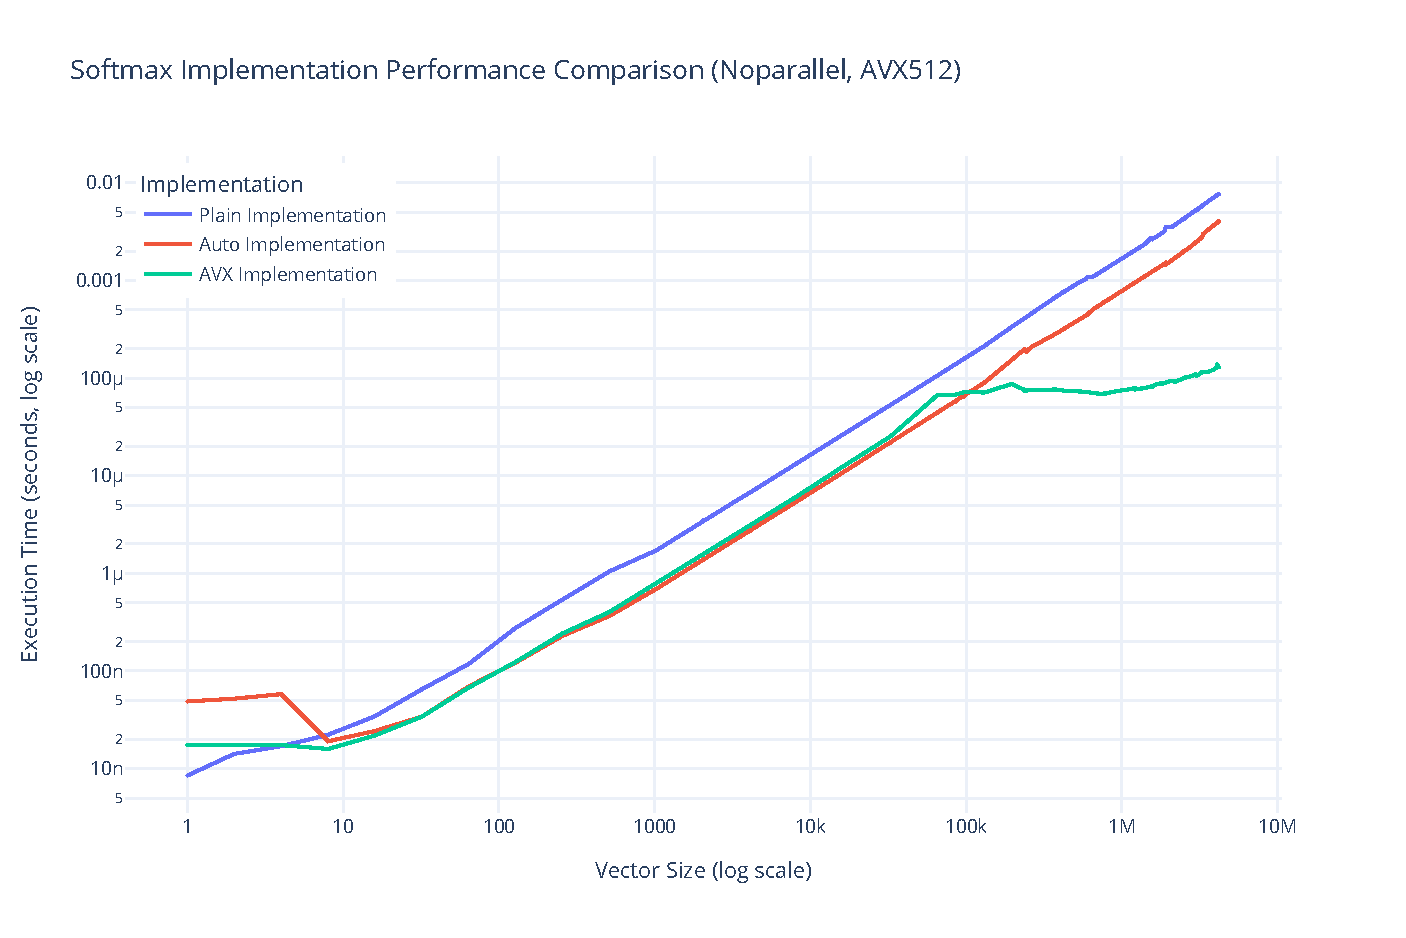
\includegraphics[width=\textwidth]{../images/performance/softmax_noparallel_avx512.pdf}
    \caption{Performance of softmax implementations without parallelization and with AVX512 instructions.}
    \label{fig:perf_noparallel_avx512}
  \end{minipage}
  \hfill
  \begin{minipage}{0.48\textwidth}
    \centering
    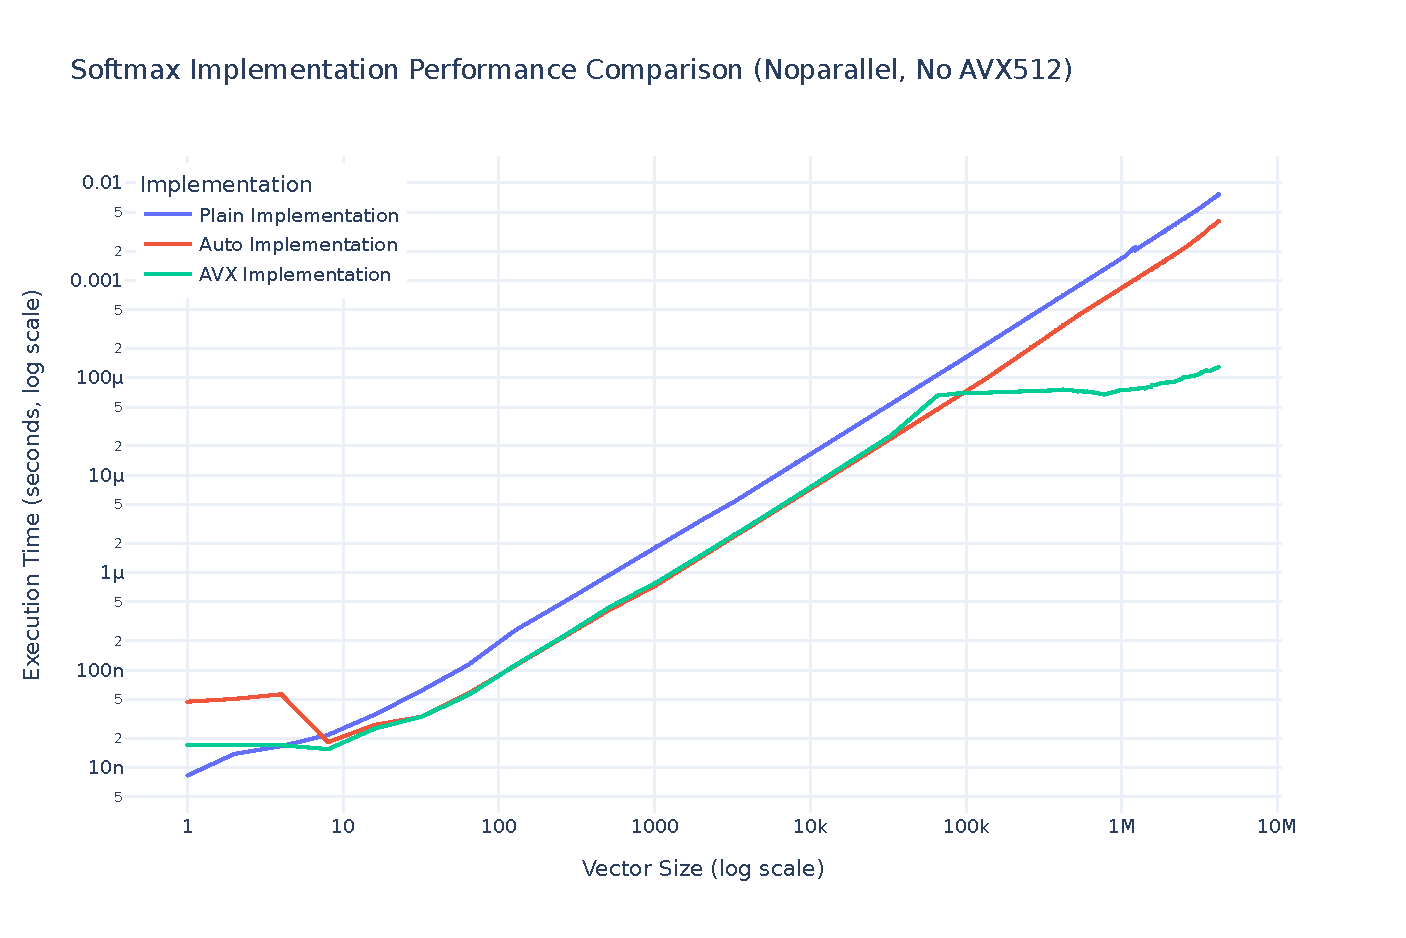
\includegraphics[width=\textwidth]{../images/performance/softmax_noparallel_noavx512.pdf}
    \caption{Performance of softmax implementations without parallelization and without AVX512 instructions.}
    \label{fig:perf_noparallel_noavx512}
  \end{minipage}
\end{figure}

\begin{figure}[H]
  \centering
  \begin{minipage}{0.48\textwidth}
    \centering
    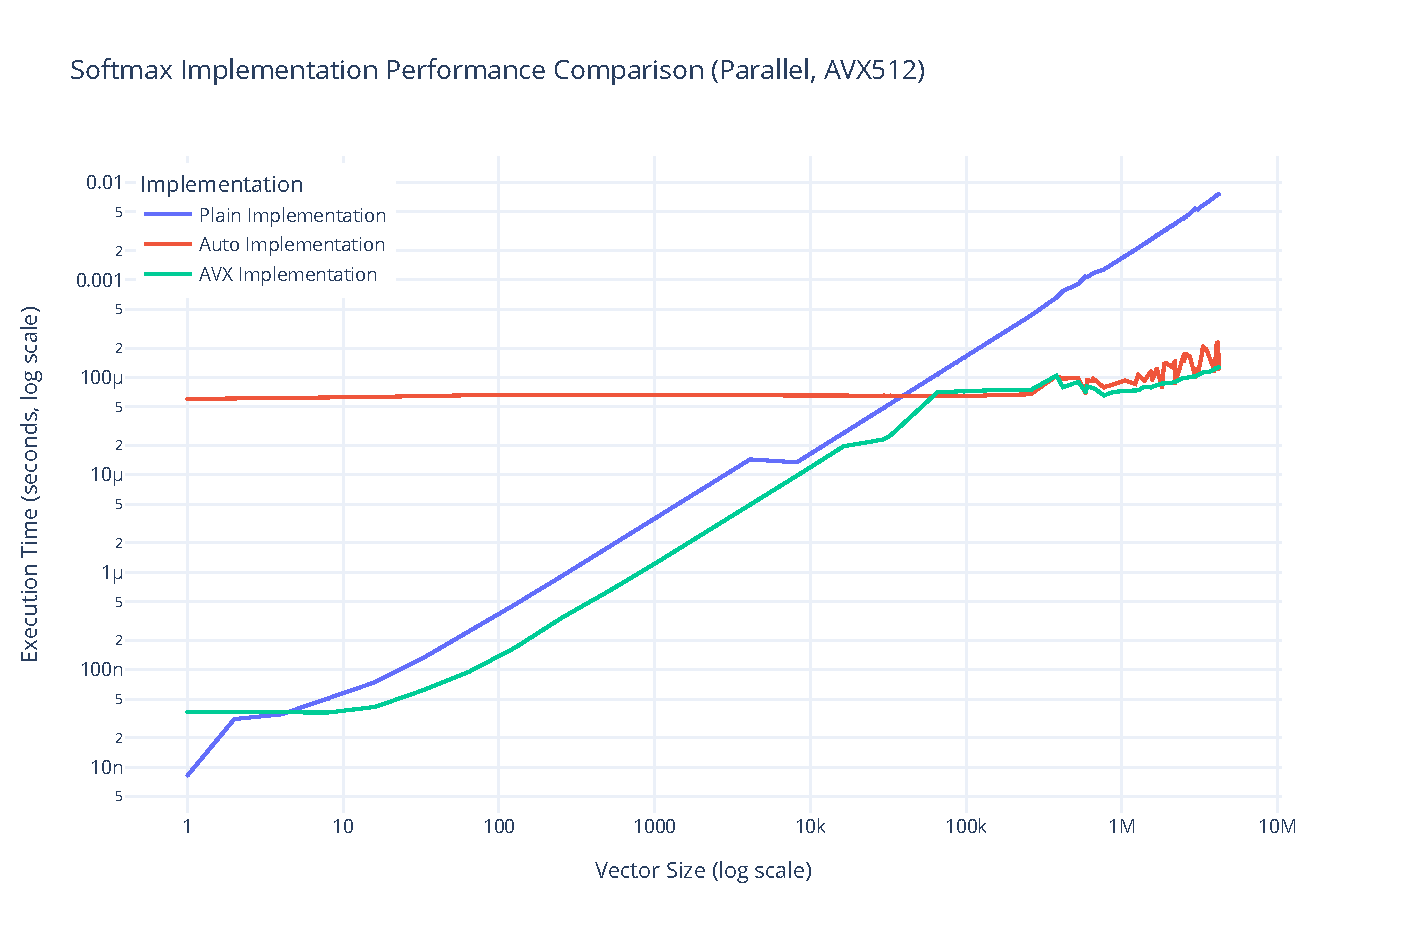
\includegraphics[width=\textwidth]{../images/performance/softmax_parallel_avx512.pdf}
    \caption{Performance of softmax implementations with parallelization and AVX512 instructions.}
    \label{fig:perf_parallel_avx512}
  \end{minipage}
  \hfill
  \begin{minipage}{0.48\textwidth}
    \centering
    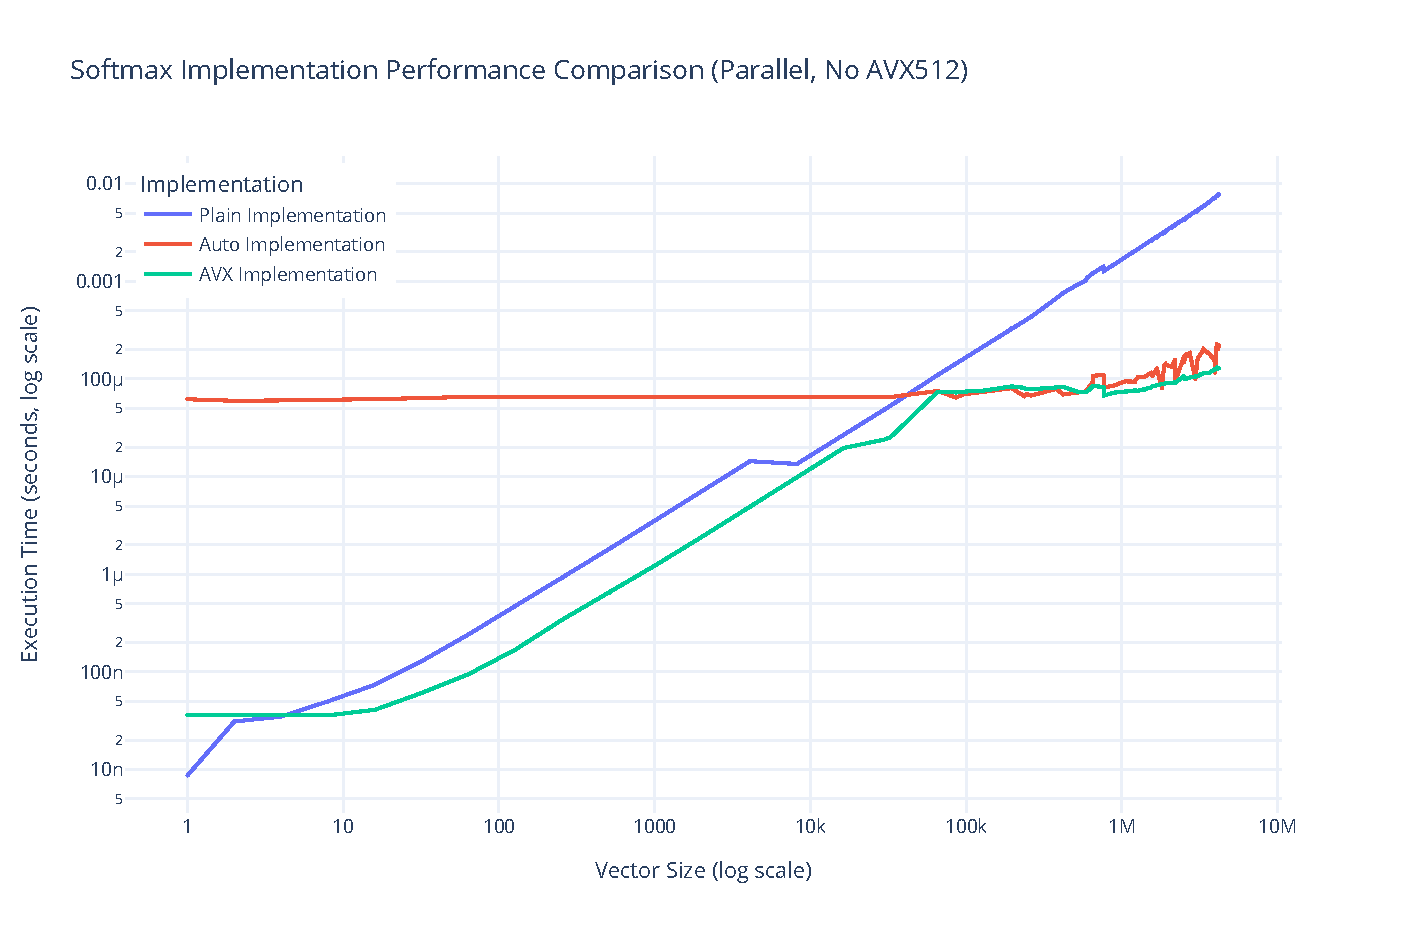
\includegraphics[width=\textwidth]{../images/performance/softmax_parallel_noavx512.pdf}
    \caption{Performance of softmax implementations with parallelization but without AVX512 instructions.}
    \label{fig:perf_parallel_noavx512}
  \end{minipage}
\end{figure}

\subsection*{Speedup}
We analyze the relative speedup of various configurations compared to the baseline plain implementation. Figures~\ref{fig:speedup_parallel_avx512} through \ref{fig:speedup_noparallel_noavx512} illustrate the performance gains achieved through different combinations of parallelization and vectorization techniques.

\begin{figure}[H]
  \centering
  \begin{minipage}{0.48\textwidth}
    \centering
    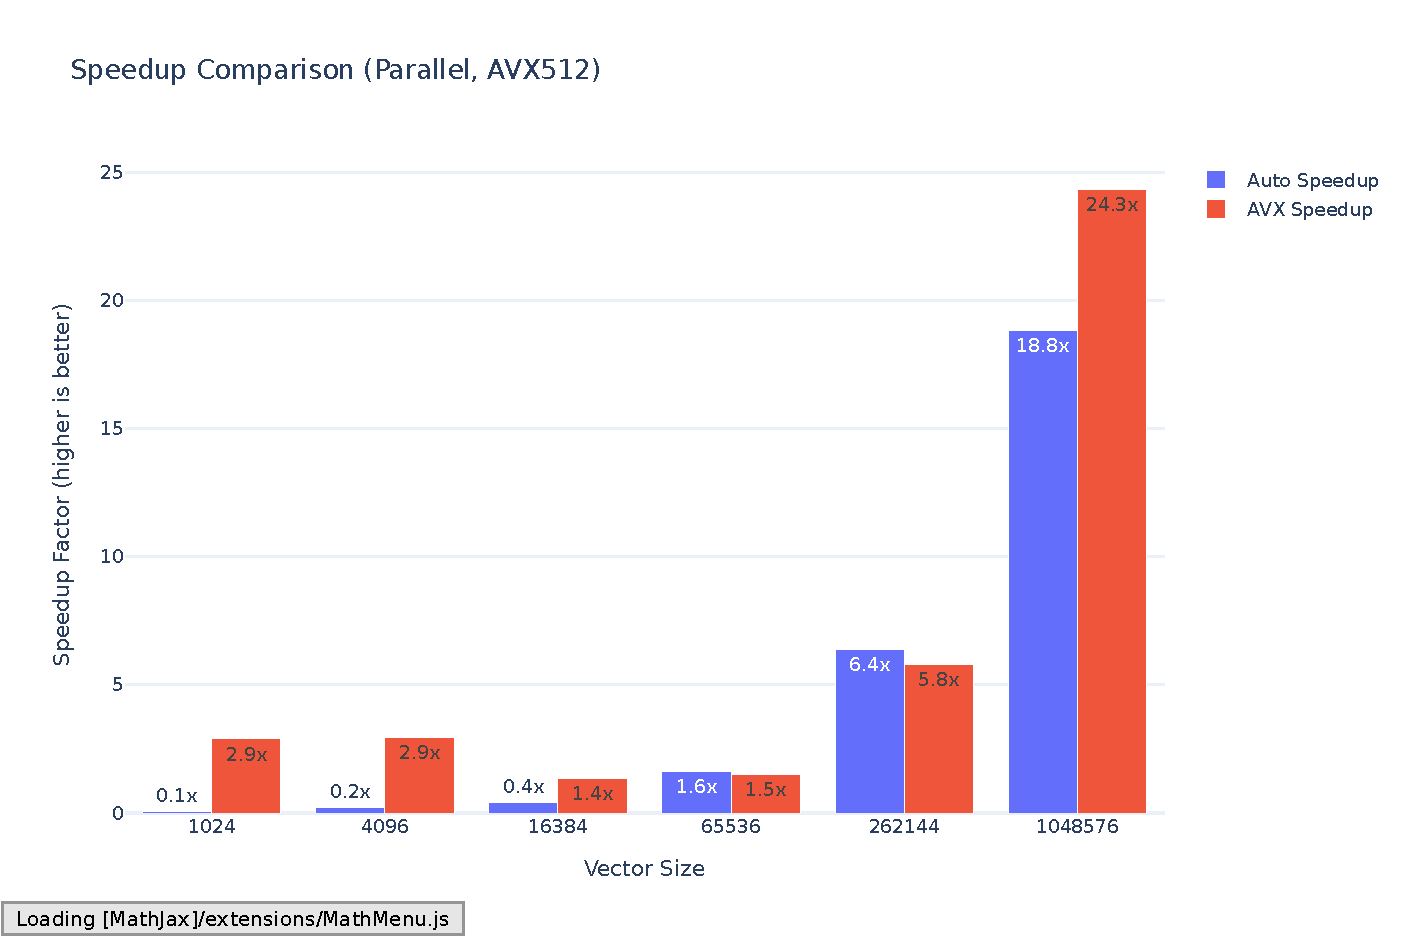
\includegraphics[width=\textwidth]{../images/speedup/softmax_speedup_parallel_avx512.pdf}
    \caption{Speedup with parallelization and AVX512 instructions.}
    \label{fig:speedup_parallel_avx512}
  \end{minipage}
  \hfill
  \begin{minipage}{0.48\textwidth}
    \centering
    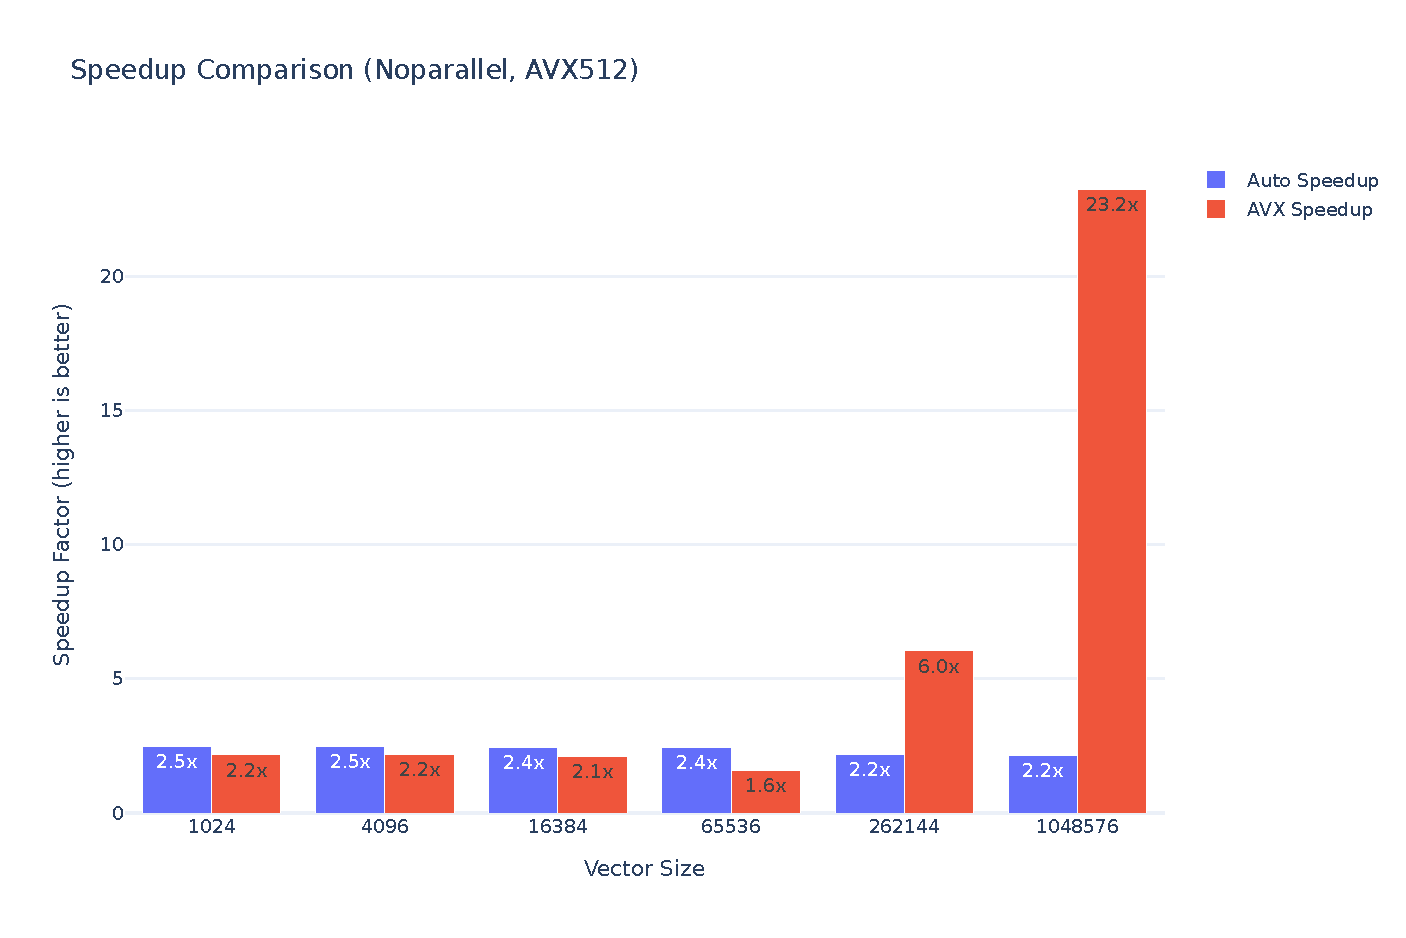
\includegraphics[width=\textwidth]{../images/speedup/softmax_speedup_noparallel_avx512.pdf}
    \caption{Speedup without parallelization but with AVX512 instructions.}
    \label{fig:speedup_noparallel_avx512}
  \end{minipage}
\end{figure}

\begin{figure}[H]
  \centering
  \begin{minipage}{0.48\textwidth}
    \centering
    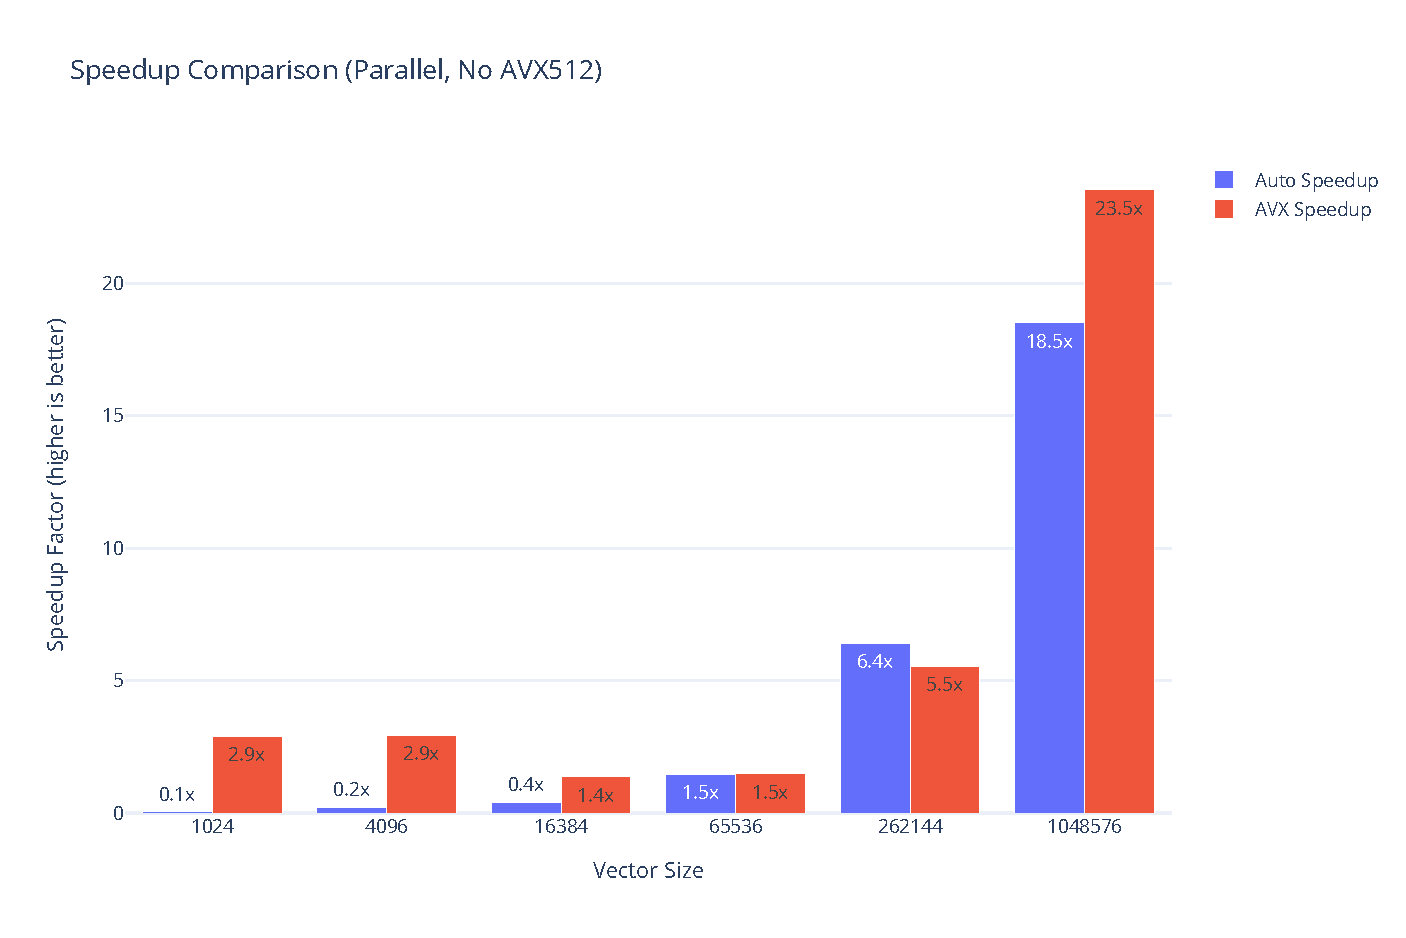
\includegraphics[width=\textwidth]{../images/speedup/softmax_speedup_parallel_noavx512.pdf}
    \caption{Speedup with parallelization but without AVX512 instructions.}
    \label{fig:speedup_parallel_noavx512}
  \end{minipage}
  \hfill
  \begin{minipage}{0.48\textwidth}
    \centering
    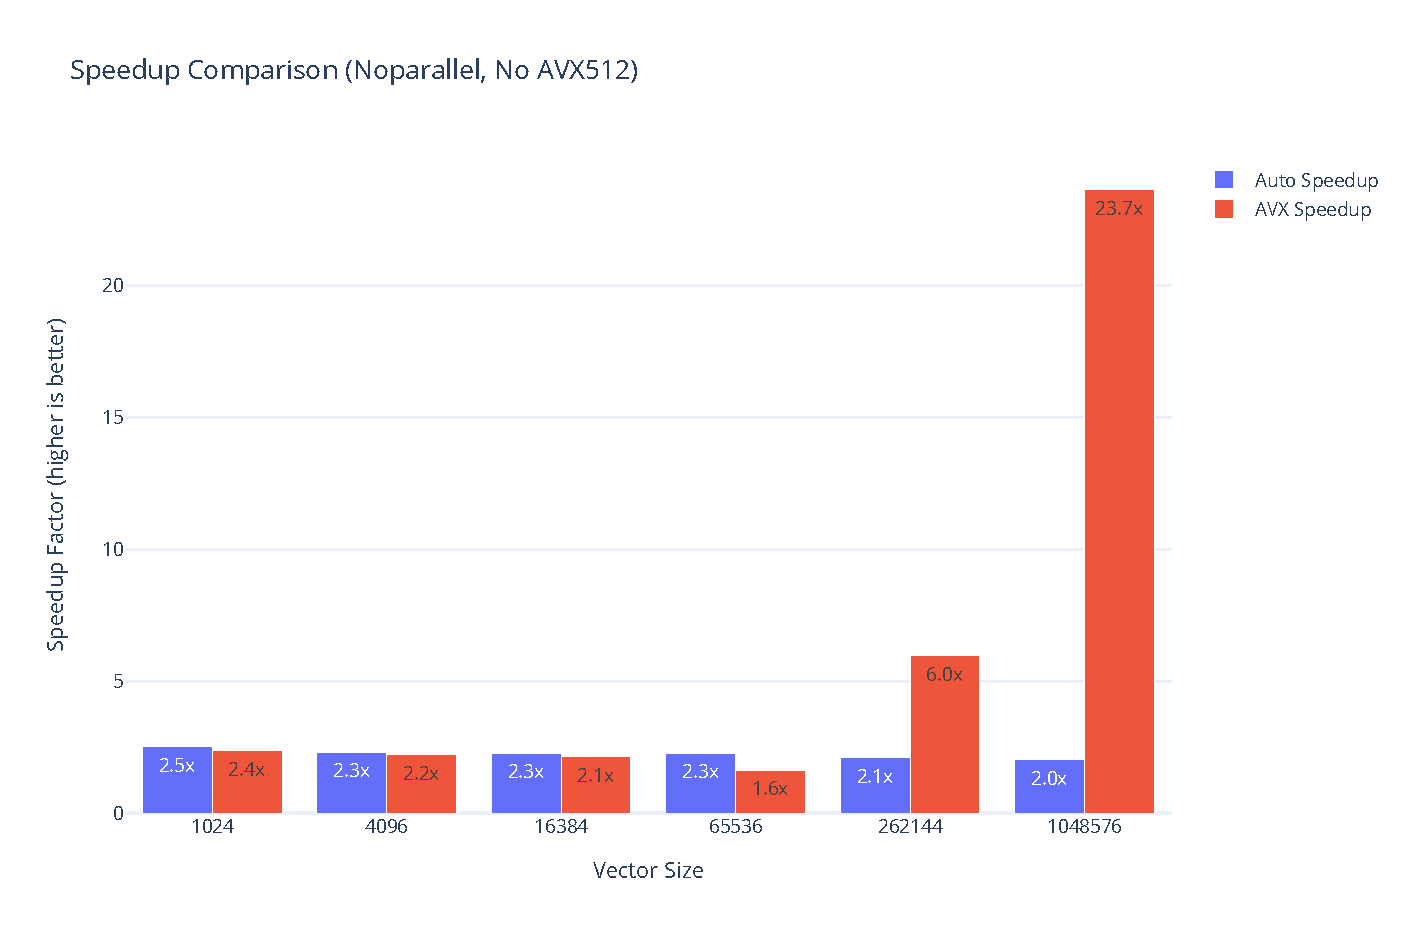
\includegraphics[width=\textwidth]{../images/speedup/softmax_speedup_noparallel_noavx512.pdf}
    \caption{Speedup without parallelization and without AVX512 instructions.}
    \label{fig:speedup_noparallel_noavx512}
  \end{minipage}
\end{figure}

As evidenced in Figures~\ref{fig:speedup_parallel_avx512} and \ref{fig:speedup_parallel_noavx512}, parallelization significantly enhances the performance of the auto-vectorized implementation. Conversely, the impact of AVX512 instructions appears minimal when comparing Figures~\ref{fig:speedup_parallel_avx512} with \ref{fig:speedup_parallel_noavx512} and \ref{fig:speedup_noparallel_avx512} with \ref{fig:speedup_noparallel_noavx512}.

\subsection*{Scalability}

We evaluate thread scalability using a fixed large input size ($K = 2^{30}$) while varying thread count from 1 to 96. Figure~\ref{fig:thread_scaling} shows the execution times, while Figure~\ref{fig:thread_speedup} presents the speedup relative to single-threaded execution alongside the theoretical Amdahl's Law prediction. Notably, a performance discontinuity occurs at approximately half the maximum thread count, corresponding to the number of cores in one of the system's two physical processors.

\begin{figure}[H]
  \centering
  \begin{minipage}{0.48\textwidth}
    \centering
    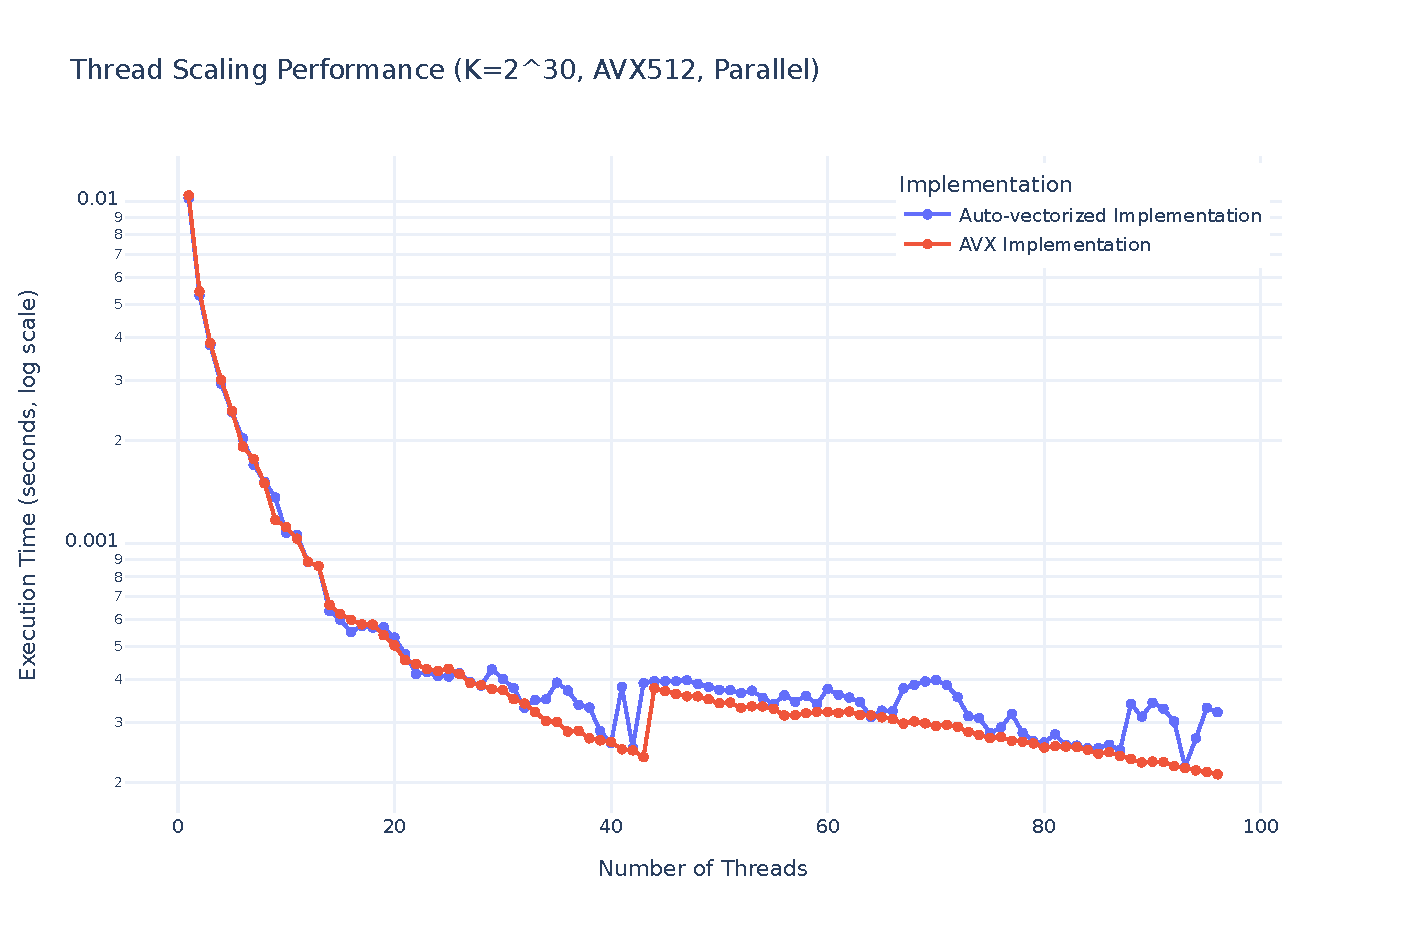
\includegraphics[width=\textwidth]{../images/thread_scaling/thread_scaling_avx512.pdf}
    \caption{Execution time scaling with thread count for the softmax implementations.}
    \label{fig:thread_scaling}
  \end{minipage}
  \hfill
  \begin{minipage}{0.48\textwidth}
    \centering
    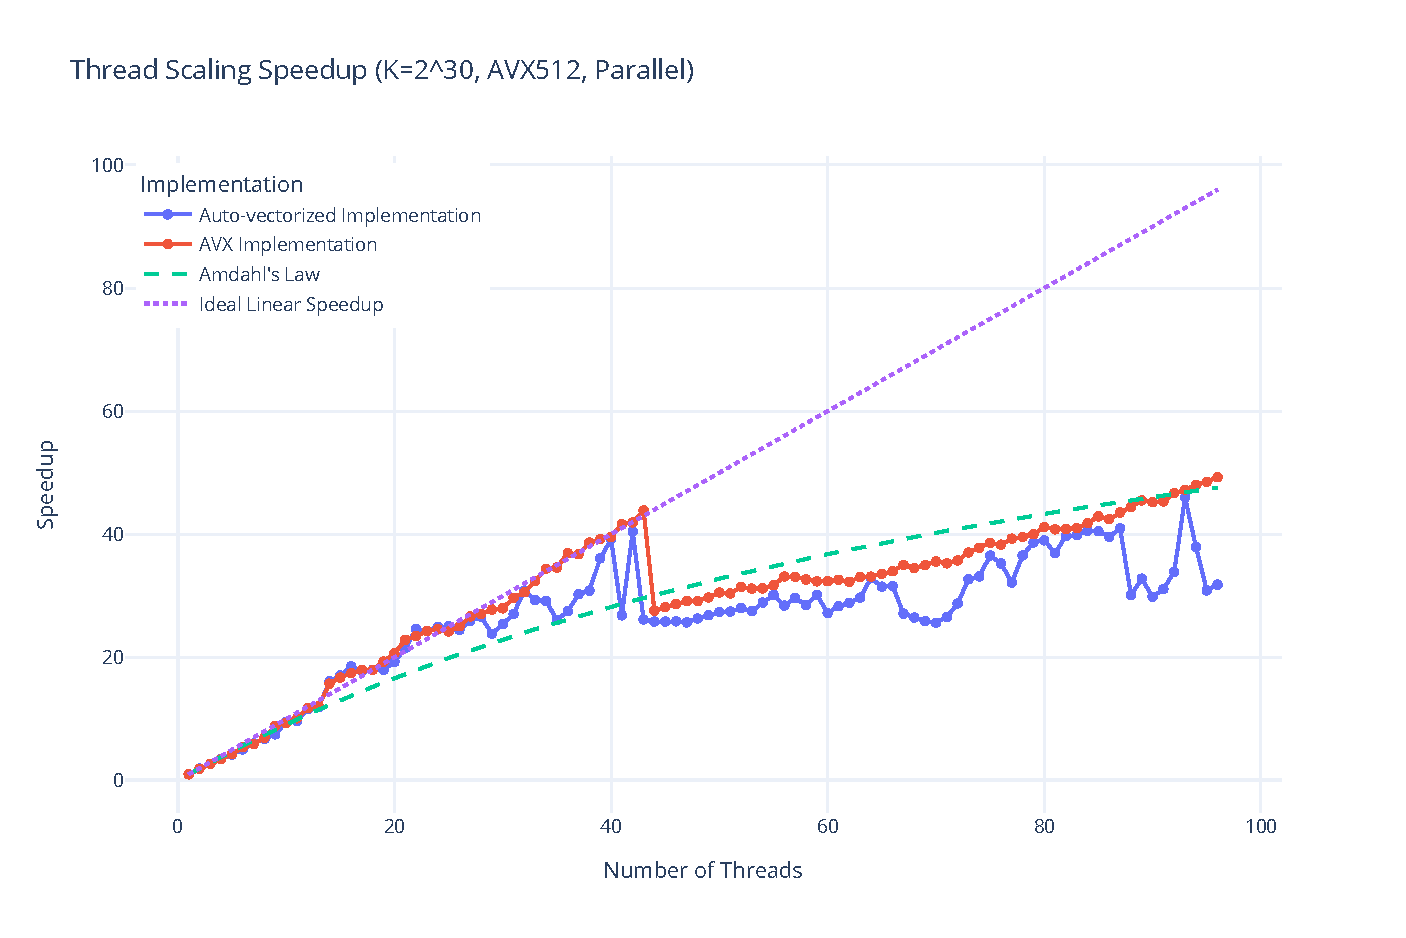
\includegraphics[width=\textwidth]{../images/thread_scaling/thread_scaling_speedup_avx512.pdf}
    \caption{Thread scaling speedup compared to Amdahl's Law prediction.}
    \label{fig:thread_speedup}
  \end{minipage}
\end{figure}

\subsection*{Numerical Stability}
The numerical stability comparison in Figures~\ref{fig:stability_noparallel} and \ref{fig:stability_parallel} demonstrates how each implementation handles numerical challenges across varying input conditions.

\begin{figure}[H]
  \centering
  \begin{minipage}{0.48\textwidth}
    \centering
    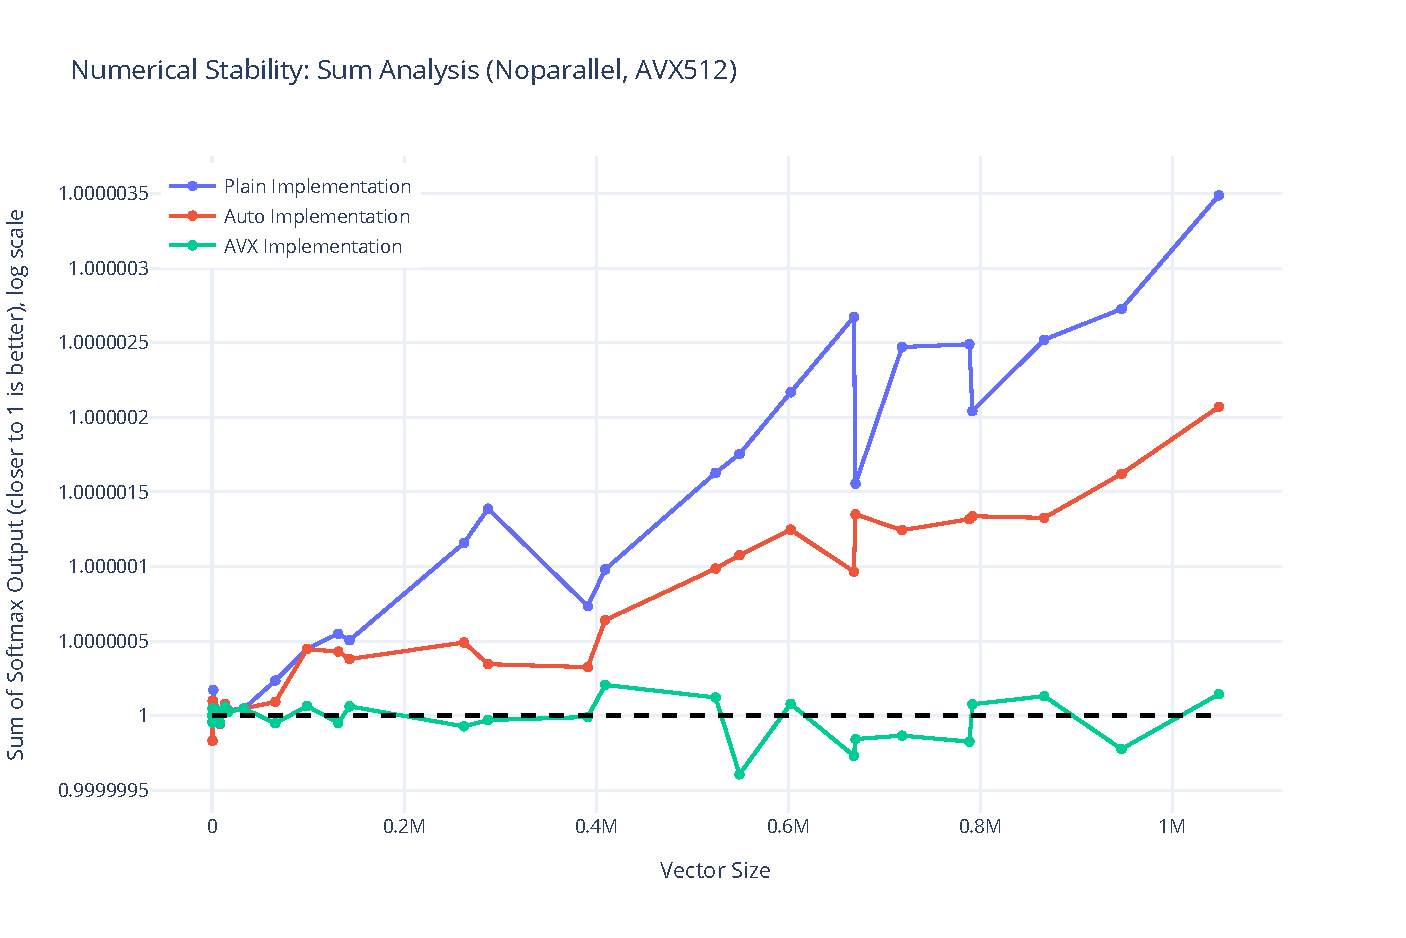
\includegraphics[width=\textwidth]{../images/stability/stability_noparallel_avx512.pdf}
    \caption{Numerical stability without parallelization.}
    \label{fig:stability_noparallel}
  \end{minipage}
  \hfill
  \begin{minipage}{0.48\textwidth}
    \centering
    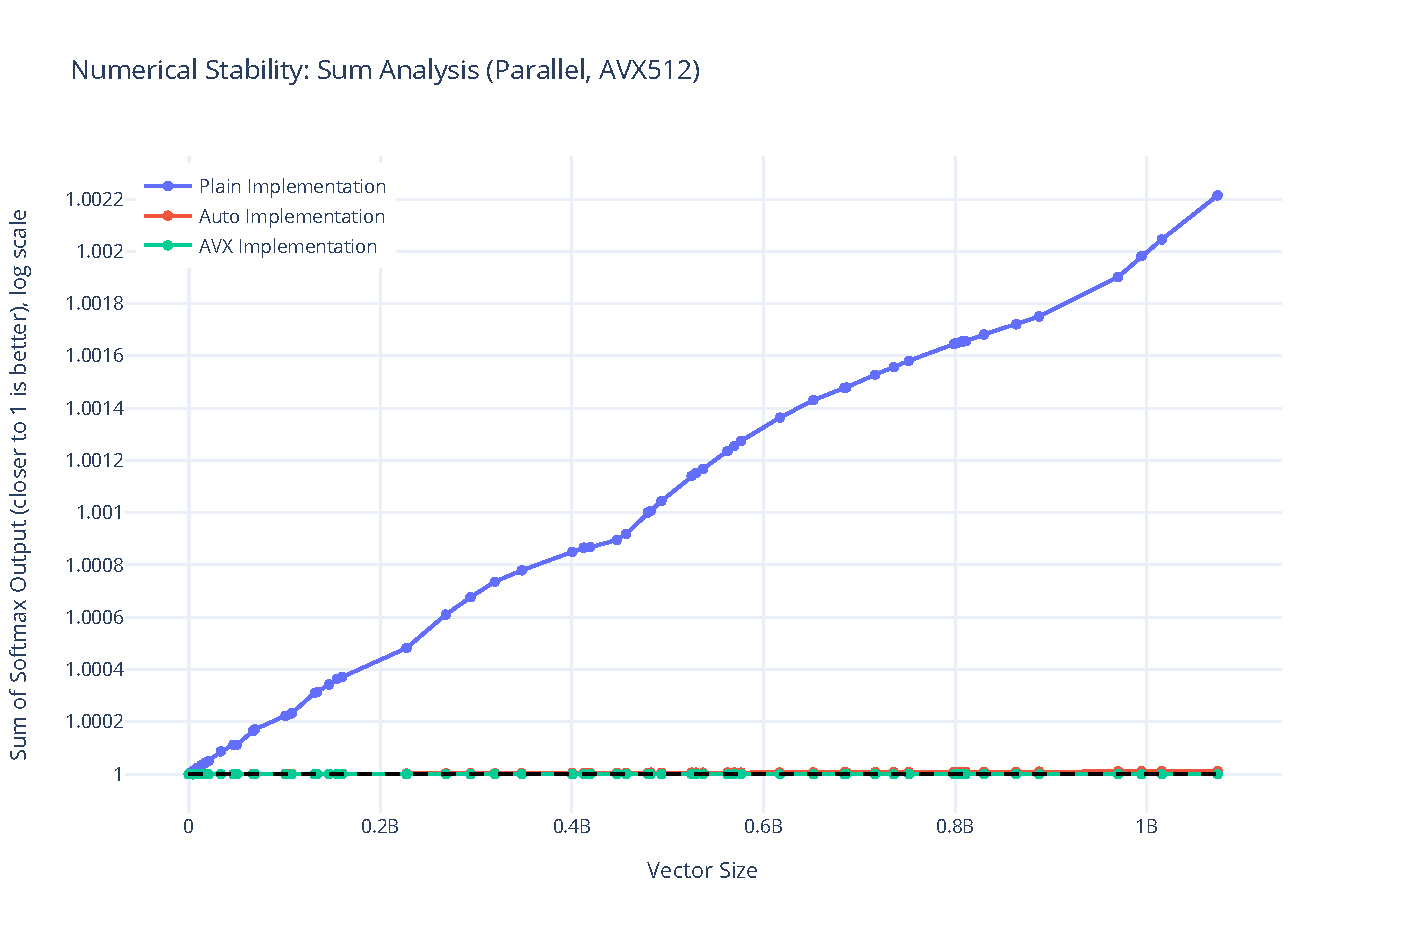
\includegraphics[width=\textwidth]{../images/stability/stability_parallel_avx512.pdf}
    \caption{Numerical stability with parallelization.}
    \label{fig:stability_parallel}
  \end{minipage}
\end{figure}

\end{document}
